\section{MaskedBiMamba for skeleton-based fall detection}
\label{sec:method}

\subsection{Pose representation and temporal windows}

MaskedBiMamba receives a sequence of estimated poses of one person. We retain $J=12$ body joints, excluding the five facial keypoints. Let $r_{t,j}^{(a)}$ be joint $j$'s coordinate along axis $a\in\{x,y\}$ at time $t$, and $c_{t,j}\in[0,1]$ its confidence. Each axis is normalized within a frame:
\begin{equation}
    \bar r_{t,j}^{(a)}=
    \frac{r_{t,j}^{(a)}-\min_k r_{t,k}^{(a)}}
    {\max\!\left(\max_k r_{t,k}^{(a)}-\min_k r_{t,k}^{(a)},10^{-4}\right)}.
    \label{eq:pose_normalization}
\end{equation}
The frame vector $\mathbf x_t=[\bar r_{t,j}^{(x)},\bar r_{t,j}^{(y)},c_{t,j}]_{j=1}^{J}\in\mathbb R^{36}$ describes relative body configuration and joint confidence. Per-frame normalization reduces dependence on image position and body scale. A separate quality vector records the mean joint confidence, visible-joint fraction, and person-box confidence $b_t$:
\begin{equation}
    \mathbf q_t=
    \left[\frac{1}{J}\sum_{j=1}^{J}c_{t,j},\;
    \frac{1}{J}\sum_{j=1}^{J}\mathbb I(c_{t,j}\geq0.2),\;b_t\right]^{\!\top}.
    \label{eq:quality_features}
\end{equation}
Here $\mathbb I(\cdot)$ is the indicator function.

Each input window spans 1.0~s and is linearly interpolated to $T=30$ time steps. Successive windows advance by 0.2~s.

\subsection{Masked input and temporal attention}

MaskedBiMamba combines frame masking, temporal attention, bidirectional Mamba stacks, and quality-weighted pooling (Fig.~\ref{fig:masked_bimamba}). The architecture relates observations before and after a posture change while retaining pose quality as a separate input. The selective state-space operator itself follows Mamba~\cite{gu2023mamba}.

During training, a Bernoulli variable $m_t$ determines whether the pose at time $t$ is retained. The masked pose is embedded in $d=64$ dimensions:
\begin{equation}
    m_t\sim\operatorname{Bernoulli}(1-\rho),\qquad
    \mathbf e_t=\mathbf W_e(m_t\mathbf x_t)+\mathbf b_e+\mathbf p_t,
    \label{eq:masked_embedding}
\end{equation}
where $\rho=0.15$, $\mathbf W_e\in\mathbb R^{d\times36}$, $\mathbf b_e\in\mathbb R^d$, and $\mathbf p_t\in\mathbb R^d$ is a learned position embedding. If every frame is masked, the first is retained. Training-time masking exposes the classifier to windows with missing frame observations. The quality stream remains unchanged; inference uses $m_t=1$ for every frame.

Stacking $\mathbf e_t^\top$ gives $\mathbf E\in\mathbb R^{T\times d}$. Four attention heads compare all positions within the window. For head $k$, with $d_h=d/4=16$,
\begin{equation}
    \mathbf A_k=\operatorname{softmax}\!\left(
    \frac{(\mathbf E\mathbf W_k^Q)(\mathbf E\mathbf W_k^K)^\top}
    {\sqrt{d_h}}\right)(\mathbf E\mathbf W_k^V),
    \label{eq:temporal_attention}
\end{equation}
where the softmax acts along each row and $\mathbf W_k^Q,\mathbf W_k^K,\mathbf W_k^V\in\mathbb R^{d\times d_h}$ are learned projections. The attended sequence is
\begin{equation}
    \mathbf H=\operatorname{LN}\!\left(
    \mathbf E+[\mathbf A_1\Vert\cdots\Vert\mathbf A_4]\mathbf W^O
    \right),
    \label{eq:attention_residual}
\end{equation}
where $\Vert$ denotes feature concatenation, $\mathbf W^O\in\mathbb R^{d\times d}$, and $\operatorname{LN}$ is layer normalization. Affine projection biases are omitted in Eqs.~\eqref{eq:temporal_attention} and~\eqref{eq:attention_residual} for readability. Attention connects observations at different positions before the recurrent state updates.

\subsection{Selective state space and bidirectional fusion}

Mamba's selective state-space update makes its step size and input/output coefficients depend on the current feature~\cite{gu2023mamba}. We retain the standard Mamba input projection, causal depthwise convolution, SiLU gate, selective scan, and output projection. Each block uses state size 16, convolution width 4, and expansion factor 2, giving 128 internal channels. Our architectural change consists of independent forward and backward processing. The underlying Mamba operator is retained without a change to its selective update.

To use both temporal directions, independent forward and backward stacks process the same attended window. Let $\mathcal R$ reverse the time axis, and let $\mathcal M_f^{(\ell)}$ and $\mathcal M_b^{(\ell)}$ denote the Mamba blocks at layer $\ell$. Starting with $\mathbf F^{(0)}=\mathbf H$ and $\mathbf B^{(0)}=\mathcal R(\mathbf H)$, the two residual stacks compute
\begin{equation}
    \begin{aligned}
        \mathbf F^{(\ell)}&=\mathbf F^{(\ell-1)}+
        \mathcal M_f^{(\ell)}(\mathbf F^{(\ell-1)}),\\
        \mathbf B^{(\ell)}&=\mathbf B^{(\ell-1)}+
        \mathcal M_b^{(\ell)}(\mathbf B^{(\ell-1)}),
    \end{aligned}\quad \ell=1,2.
    \label{eq:bidirectional_stacks}
\end{equation}
The reverse output is restored to the original time order before fusion:
\begin{equation}
    \mathbf H^*=\operatorname{LN}\!\left(
    [\mathbf F^{(2)}\Vert\mathcal R(\mathbf B^{(2)})]\mathbf W_f+\mathbf b_f
    \right),
    \label{eq:direction_fusion}
\end{equation}
where $\mathbf W_f\in\mathbb R^{128\times64}$ and $\mathbf b_f\in\mathbb R^{64}$. Its row $\mathbf h_t^\top$ describes time $t$ using preceding and subsequent observations in the buffered window. The aligned representation relates a descent to its subsequent posture within the buffered window. Bidirectional processing produces one classification after that window has been collected.

\begin{figure*}[tp]
    \centering
    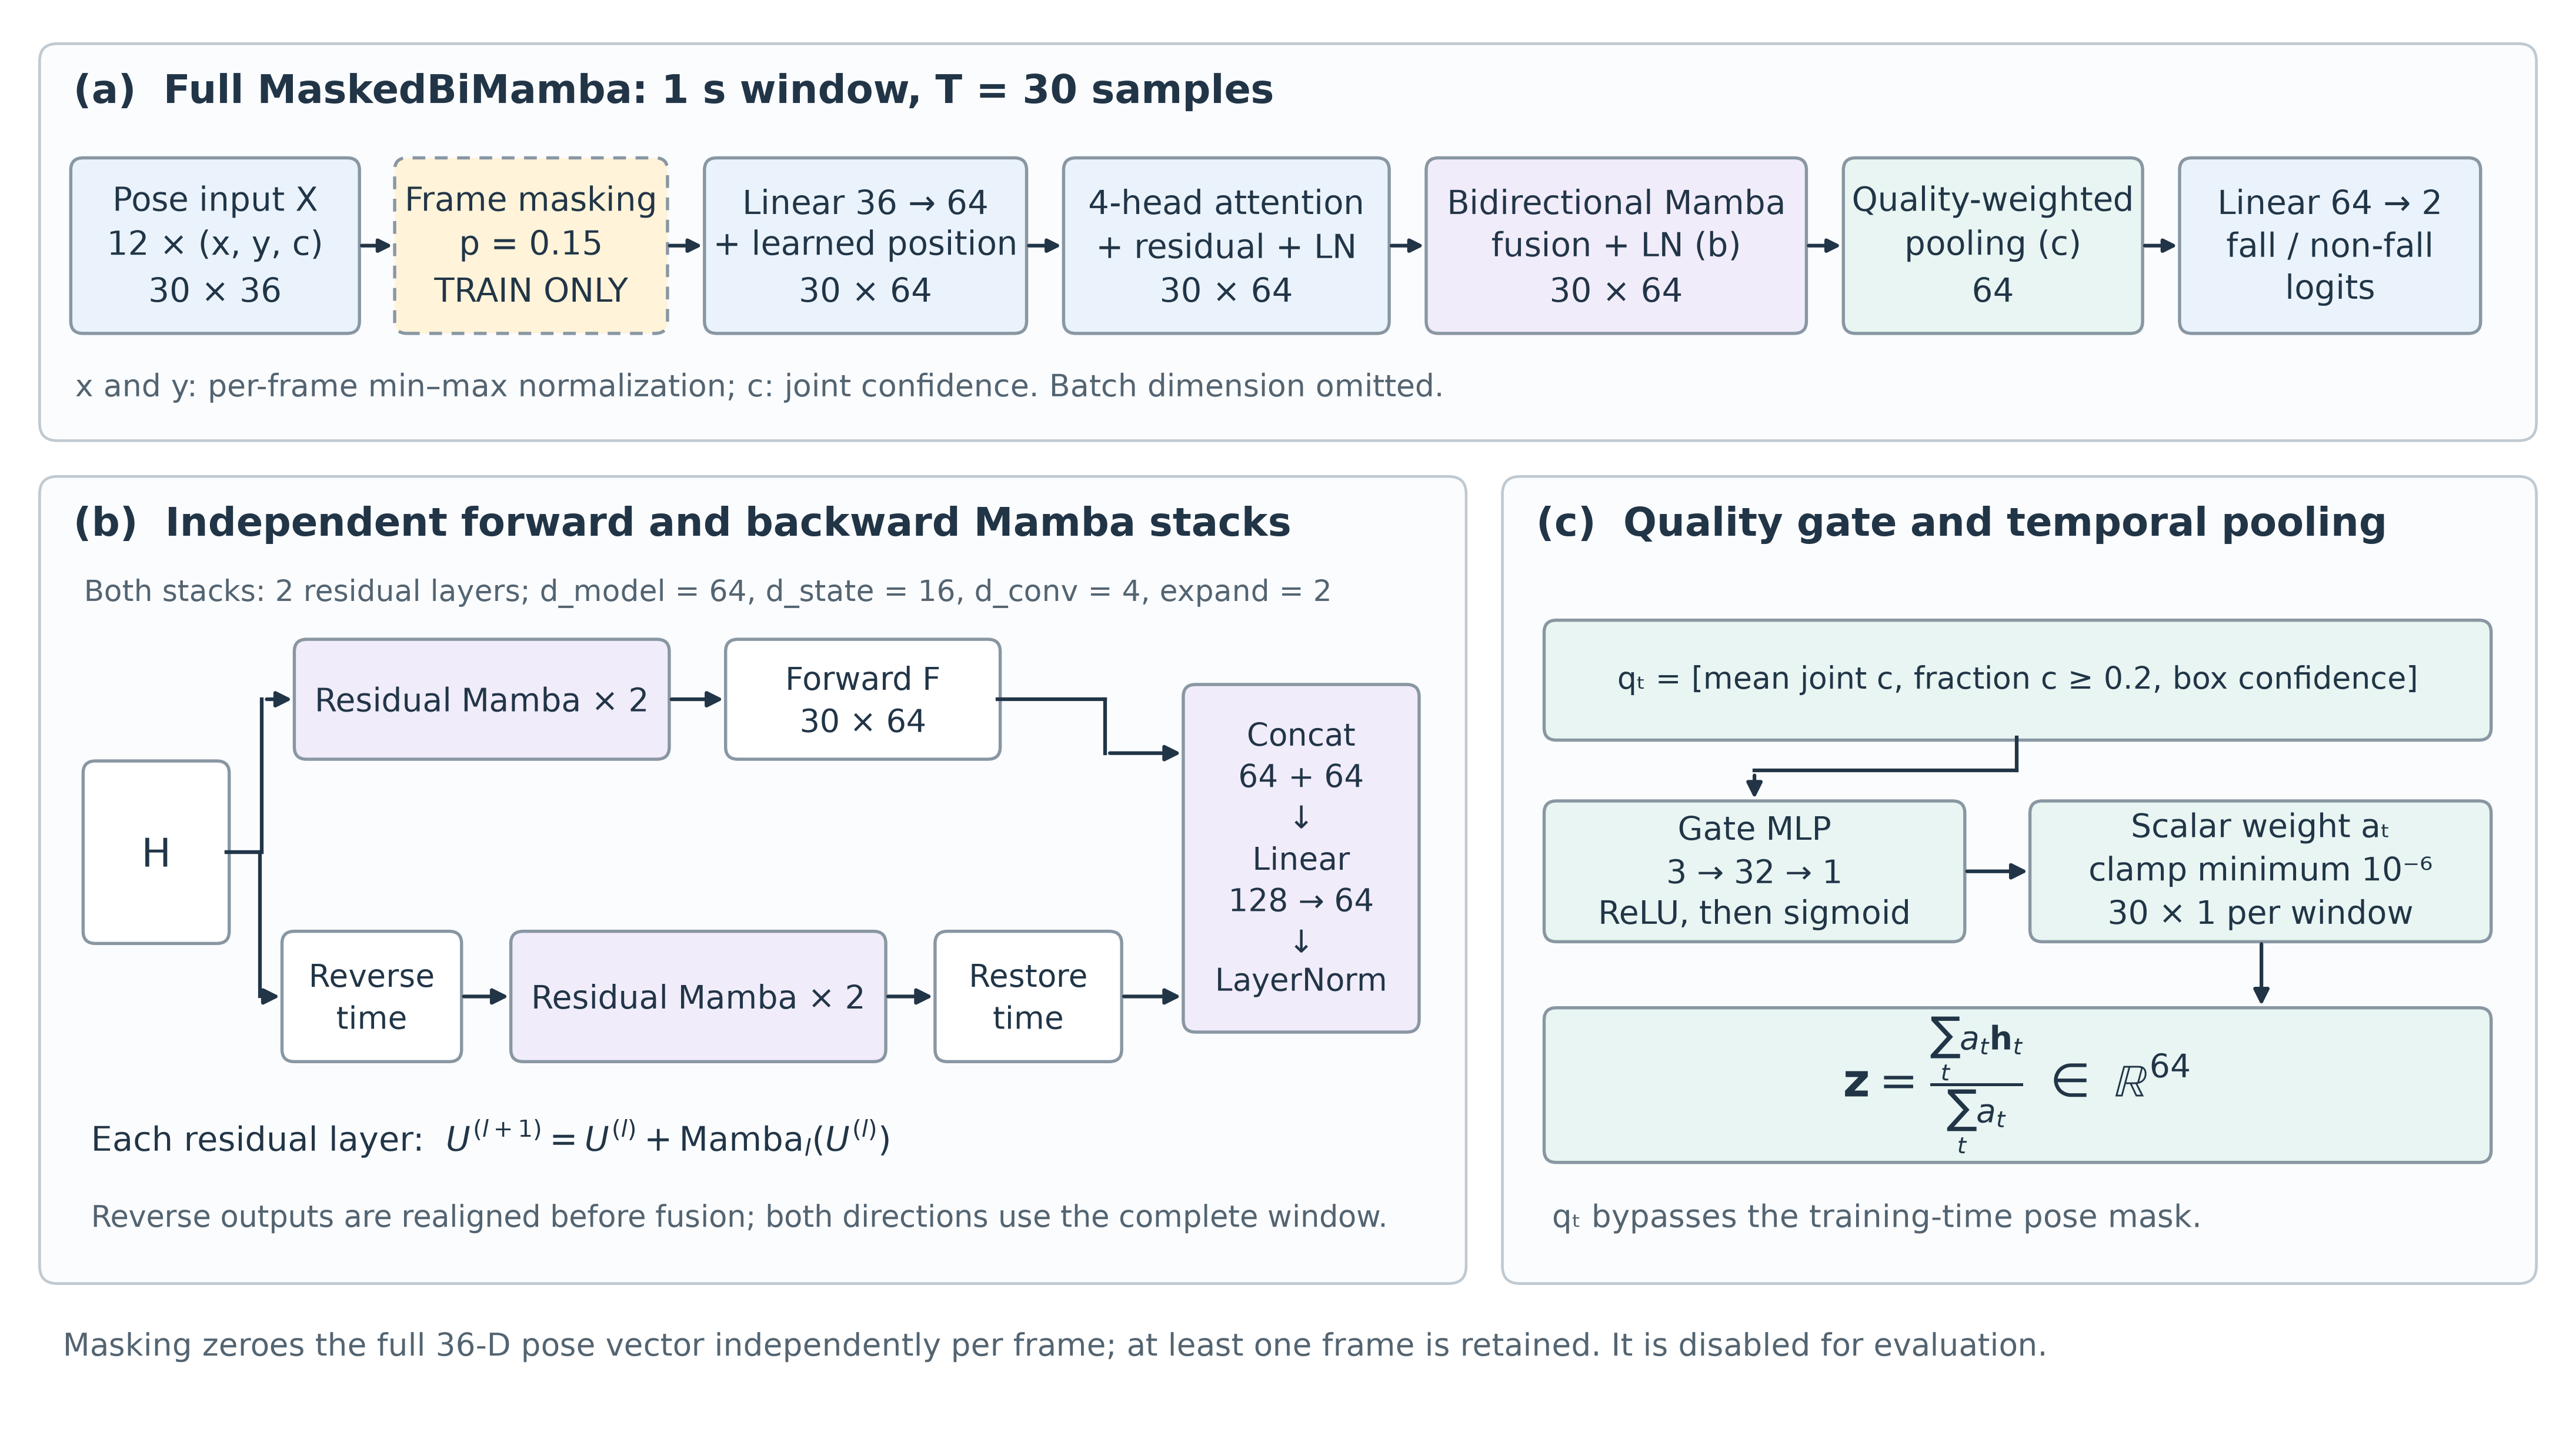
\includegraphics[width=\textwidth]{figs/masked_bimamba_architecture_reviewed.png}
    \caption{MaskedBiMamba architecture. Pose features pass through training-time frame masking, temporal attention and two independent Mamba stacks. The reverse stream is aligned before fusion. A separate quality network supplies the temporal pooling weights. Tensor dimensions omit the batch axis.}
    \label{fig:masked_bimamba}
\end{figure*}

\subsection{Quality-weighted pooling and classification}

Uniform pooling assigns the same coefficient to every frame, even when pose confidence varies. We instead learn a scalar weight from each quality vector:
\begin{equation}
    a_t=\max\!\left\{10^{-6},\,
    \sigma\!\left[\mathbf w_2^\top\operatorname{ReLU}
    (\mathbf W_1\mathbf q_t+\mathbf b_1)+b_2\right]\right\},
    \label{eq:quality_gate}
\end{equation}
where $\mathbf W_1\in\mathbb R^{32\times3}$, $\mathbf b_1,\mathbf w_2\in\mathbb R^{32}$, $b_2\in\mathbb R$, and $\sigma$ is the sigmoid function. The gate is trained jointly with the classifier. Normalizing its outputs gives
\begin{equation}
    \alpha_t=\frac{a_t}{\sum_{u=1}^{T}a_u},\qquad
    \mathbf z=\sum_{t=1}^{T}\alpha_t\mathbf h_t.
    \label{eq:quality_pooling}
\end{equation}
The coefficients satisfy $\alpha_t>0$ and $\sum_t\alpha_t=1$. These coefficients adjust each frame's contribution using the separate quality input. Equal coefficients recover temporal mean pooling over the complete window. The window representation $\mathbf z\in\mathbb R^{64}$ yields two class logits and probabilities:
\begin{equation}
    \boldsymbol\ell=\mathbf W_c\mathbf z+\mathbf b_c,\qquad
    \pi_c=\frac{e^{\ell_c}}{e^{\ell_0}+e^{\ell_1}},\quad c\in\{0,1\},
    \label{eq:classification_probability}
\end{equation}
where $\mathbf W_c\in\mathbb R^{2\times64}$, $\mathbf b_c\in\mathbb R^2$, and class 1 denotes a fall.

\subsection{Training objective}

The training set contains more non-fall than fall windows. Weighted focal loss~\cite{lin2017focal} reduces the influence of easy examples while balancing the two classes:
\begin{equation}
    \begin{aligned}
        \mathcal L&=-\frac{1}{N_b}\sum_{i=1}^{N_b}
        w_{y_i}(1-\pi_{i,y_i})^{\gamma}\log\pi_{i,y_i},\\
        w_c&=\frac{N_{\mathrm{train}}}{2N_c}.
    \end{aligned}
    \label{eq:focal_loss}
\end{equation}
Here $N_b$ is the batch size, $y_i$ is the true class, $\pi_{i,y_i}$ is its predicted probability, $N_c$ is the training count of class $c$, and $N_{\mathrm{train}}=N_0+N_1$. The exponent $\gamma$ controls the down-weighting of easy examples.
